\documentclass[11pt,a4paper]{article}
\usepackage[margin=1in]{geometry}
\usepackage[utf8]{inputenc}
\usepackage[english]{babel}
\usepackage{amsmath,amssymb}
\usepackage{graphicx}
\usepackage{microtype}
\usepackage{hyperref}

\hypersetup{
  pdftitle={Numerical Optimization of a Two-Component Field 01 Profile on a Fixed Background},
  pdfauthor={Nikolai Dereviankin},
  pdfcreator={LaTeX},
  pdfproducer={pdfTeX}
}

\setlength{\parindent}{0pt}
\setlength{\parskip}{0.75\baselineskip}
\renewcommand{\arraystretch}{1.2}
\graphicspath{{figures/}{../figures/}}
\sloppy

\title{Numerical Optimization of a Two-Component Field 01 Profile on a Fixed Background\\
\large Checkpoint v0.4: Localizers, Acceptance Gates, Coordinate Closure, and Reproducibility}
\author{Nikolai Dereviankin}
\date{}

\newcommand{\xibr}{\xi_{\mathrm{br,max}}}
\newcommand{\vac}{V}
\newcommand{\host}{H}
\newcommand{\ldiff}{L_{\Delta}}
\newcommand{\lalign}{L_{\mathrm{A}}}

\begin{document}
\maketitle

\begin{center}
\textit{Working numerical report v0.4 --- edition 2026-08-07}
\end{center}

\begin{abstract}
This report records a completed stage of restricted numerical optimization for a two-component Field 01 localizer on a fixed background. Two independent deformation channels are considered: a sign-changing difference localizer controlling the relative profile of the two components, and an aligned localizer controlling their common deformation. The function families actually used in both channels are stated explicitly, including linear, quadratic, and cubic-exponential directions. Candidates were retained only after structural and spectral-physical checks, a predicted-gain gate, matching-radius comparison, and direct verification of a branch fold. The retained result is $\xibr=2.0934591793773114\times10^{-3}$, improving checkpoint v0.3 by $1.218886\%$. Nine selected coordinates are closed under the predeclared $1\%$ direct-validation threshold. The report does not claim global optimality, introduce a fundamental action, or replace a full analysis of static backreaction or dynamical stability.
\end{abstract}

\textbf{Keywords:} Field 01; two-component localizer; fixed background; numerical optimization; branch continuation; fold; predictor; matching radius; coordinate closure; reproducibility.

\section{Status and Purpose of the Report}

This text documents a specific numerical checkpoint rather than a completed physical theory. Its purpose is to separate the result that was actually computed from the broader interpretive language of Field 01 and to present the optimization procedure in a form suitable for independent checking.

The optimization domain is a restricted family of localizers inside a previously selected two-component fixed-background problem. The background equations, boundary conditions, and solution sector remain unchanged. Only the shapes of two localizing directions within a predeclared parametric ansatz are varied.

The quantity $\xibr$ is an internal dimensionless diagnostic for the maximum of a connected backreaction branch. It is not an experimentally measured observable and is not identified here with mass, charge, particle-existence probability, or any other physical observable.

\section{Restricted Profile Space}

Let $\host\in[0,1]$ denote the normalized host variable, and define
\begin{equation}
\vac(\host)=1-\host^2
\end{equation}
as the corresponding distance from the vacuum edge in profile space. Within the adopted parametric family, deformations are separated into difference and aligned channels.

\subsection{Difference Localizer}

The sign-changing localizer is written as
\begin{equation}
\ldiff(\host)
=\vac^q
+d\,B_{\Delta}(\host),
\label{eq:difference_localizer}
\end{equation}
where
\begin{equation}
B_{\Delta}(\host)
=A_{\Delta}\host^2\vac^s
\left(1-\zeta\host^2\right)
\left(1+c_{1,\Delta}\vac+c_{2,\Delta}\vac^2\right)
\exp\!\left(\lambda\vac^3\right).
\label{eq:difference_basis}
\end{equation}

The normalization is fixed by
\begin{equation}
A_{\Delta}^{-1}
=\max_{\host\in[0,1]}
\left|
\host^2\vac^s
\left(1-\zeta\host^2\right)
\left(1+c_{1,\Delta}\vac+c_{2,\Delta}\vac^2\right)
\exp\!\left(\lambda\vac^3\right)
\right|.
\end{equation}

The parameter $q$ controls the stiffness of the central core profile, $d$ is the weight of the sign-changing shoulder, $\zeta$ fixes the internal node, $s$ controls shoulder decay near the vacuum edge, $c_{1,\Delta}$ and $c_{2,\Delta}$ control the linear and quadratic widths, and $\lambda$ is a nonpolynomial cubic-exponential tilt.

\subsection{Aligned Localizer}

The aligned channel is
\begin{equation}
\lalign(\host)
=A_{\mathrm{A}}\host^2\vac^p
\left(1+c_{1,\mathrm{A}}\vac+c_{2,\mathrm{A}}\vac^2\right)
\exp\!\left(\rho\vac^3\right),
\label{eq:aligned_localizer}
\end{equation}
with
\begin{equation}
A_{\mathrm{A}}^{-1}
=\max_{\host\in[0,1]}
\left[
\host^2\vac^p
\left(1+c_{1,\mathrm{A}}\vac+c_{2,\mathrm{A}}\vac^2\right)
\exp\!\left(\rho\vac^3\right)
\right].
\end{equation}

Here $p$ controls the shell power, $c_{1,\mathrm{A}}$ and $c_{2,\mathrm{A}}$ are polynomial width directions, and $\rho$ is an independent cubic-exponential tilt of the aligned profile.

The functions in Eqs.~\eqref{eq:difference_localizer} and \eqref{eq:aligned_localizer} are parametric localizers within the selected numerical problem. They are not declared to be fundamental fields and do not by themselves define an action for the model.

Profiles of this general kind have established analogues in vortex and nontopological-soliton problems, but existence and stability of a localized solution depend on the specific action and do not follow from the ansatz shape alone \cite{derrick1964,nielsen1973,coleman1985}.

\section{Optimization Protocol}

Optimization was performed sequentially along one parametric coordinate at a time. A new candidate was not accepted merely because its predictor exceeded the current record. Authorization of a direct fold calculation required passage through several independent gates. General numerical background for branch continuation and nonlinear boundary-value problems is given, for example, in Refs.~\cite{keller1977,ascher1995}; the present report records its own restricted implementation of these ideas.

\subsection{Structural Checks}

The checks included reality, smoothness, finite normalization, recovery of the control profile when the new coordinate vanished, and independence of the new tangent direction from already closed polynomial directions. The nonpolynomial factors $\exp(\lambda\vac^3)$ and $\exp(\rho\vac^3)$ are positive for all real parameter values, but positivity of the factor does not replace physical validation of the complete candidate.

\subsection{Fixed-Background Physical Checks}

On the fixed background, a candidate had to preserve the selected spectral sector: one admissible negative mode, a positive next mode, sufficient component fractions, coherence, aligned fraction, and localization. Values separated from the control point by a region in which these conditions fail are not treated as part of the same physically connected branch.

Stability criteria for localized nonlinear waves depend strongly on the equation class. A classical example of such model-dependent spectral analysis is the Vakhitov--Kolokolov work \cite{vakhitov1973}. Its criterion is not applied directly here and is cited only as methodological context.

\subsection{Cubic Predictor}

The amplitude coordinate used for broad screening was
\begin{equation}
x=f_{\mathrm{center}}-1,
\end{equation}
with a local response model containing no free constant term:
\begin{equation}
\xi_{\mathrm{br}}(x)
=\chi_1x+\chi_2x^2+\chi_3x^3.
\label{eq:cubic_predictor}
\end{equation}

The coefficients were fitted to four points, $x=0,0.01,0.02,0.03$, located before the measured branch turn. The first positive stationary point with a negative second derivative was used as the predicted fold. The maximum calibration error of this screening rule was below $1\%$ on the control branches.

A direct fold calculation was authorized only when the predicted gain relative to the confirmed record reached the predeclared threshold
\begin{equation}
g_{\mathrm{pred}}
=\frac{\xi_{\mathrm{pred}}}{\xi_{\mathrm{record}}}-1
\geq 0.01.
\label{eq:one_percent_gate}
\end{equation}

\subsection{Direct Fold and Matching Radii}

The finalist was tested by direct branch continuation. A maximum was classified as a fold only when neighboring points had lower values of $\xi_{\mathrm{br}}$. The check was repeated at
\begin{equation}
R\in\{30,40,50\}.
\end{equation}

Additional requirements included residual, Gauss-law, source-derivative, Hessian, and sign-changing checks, detection of a turning point at each radius, and a small relative dispersion of the result across the radii.

\section{Retained Checkpoint v0.4}

The retained profile has the following parameters:
\begin{center}
\begin{tabular}{@{}lll@{}}
\textbf{Channel} & \textbf{Parameter} & \textbf{Retained value} \\
\hline
difference & $q$ & $16$ \\
difference & $d$ & $4$ \\
difference & $s$ & $1$ \\
difference & $\zeta$ & $1.8105828289285173$ \\
difference & $c_{1,\Delta}$ & $1.20$ \\
difference & $c_{2,\Delta}$ & $0$ \\
difference & $\lambda$ & $-0.35$ \\
aligned & $p$ & $1$ \\
aligned & $c_{1,\mathrm{A}}$ & $-3.260$ \\
aligned & $c_{2,\mathrm{A}}$ & $3.041$ \\
aligned & $\rho$ & $0$ \\
\end{tabular}
\end{center}

Figure~\ref{fig:retained_localizers} shows both retained localizers in the same normalized host coordinate.

\begin{figure}[htbp]
\centering
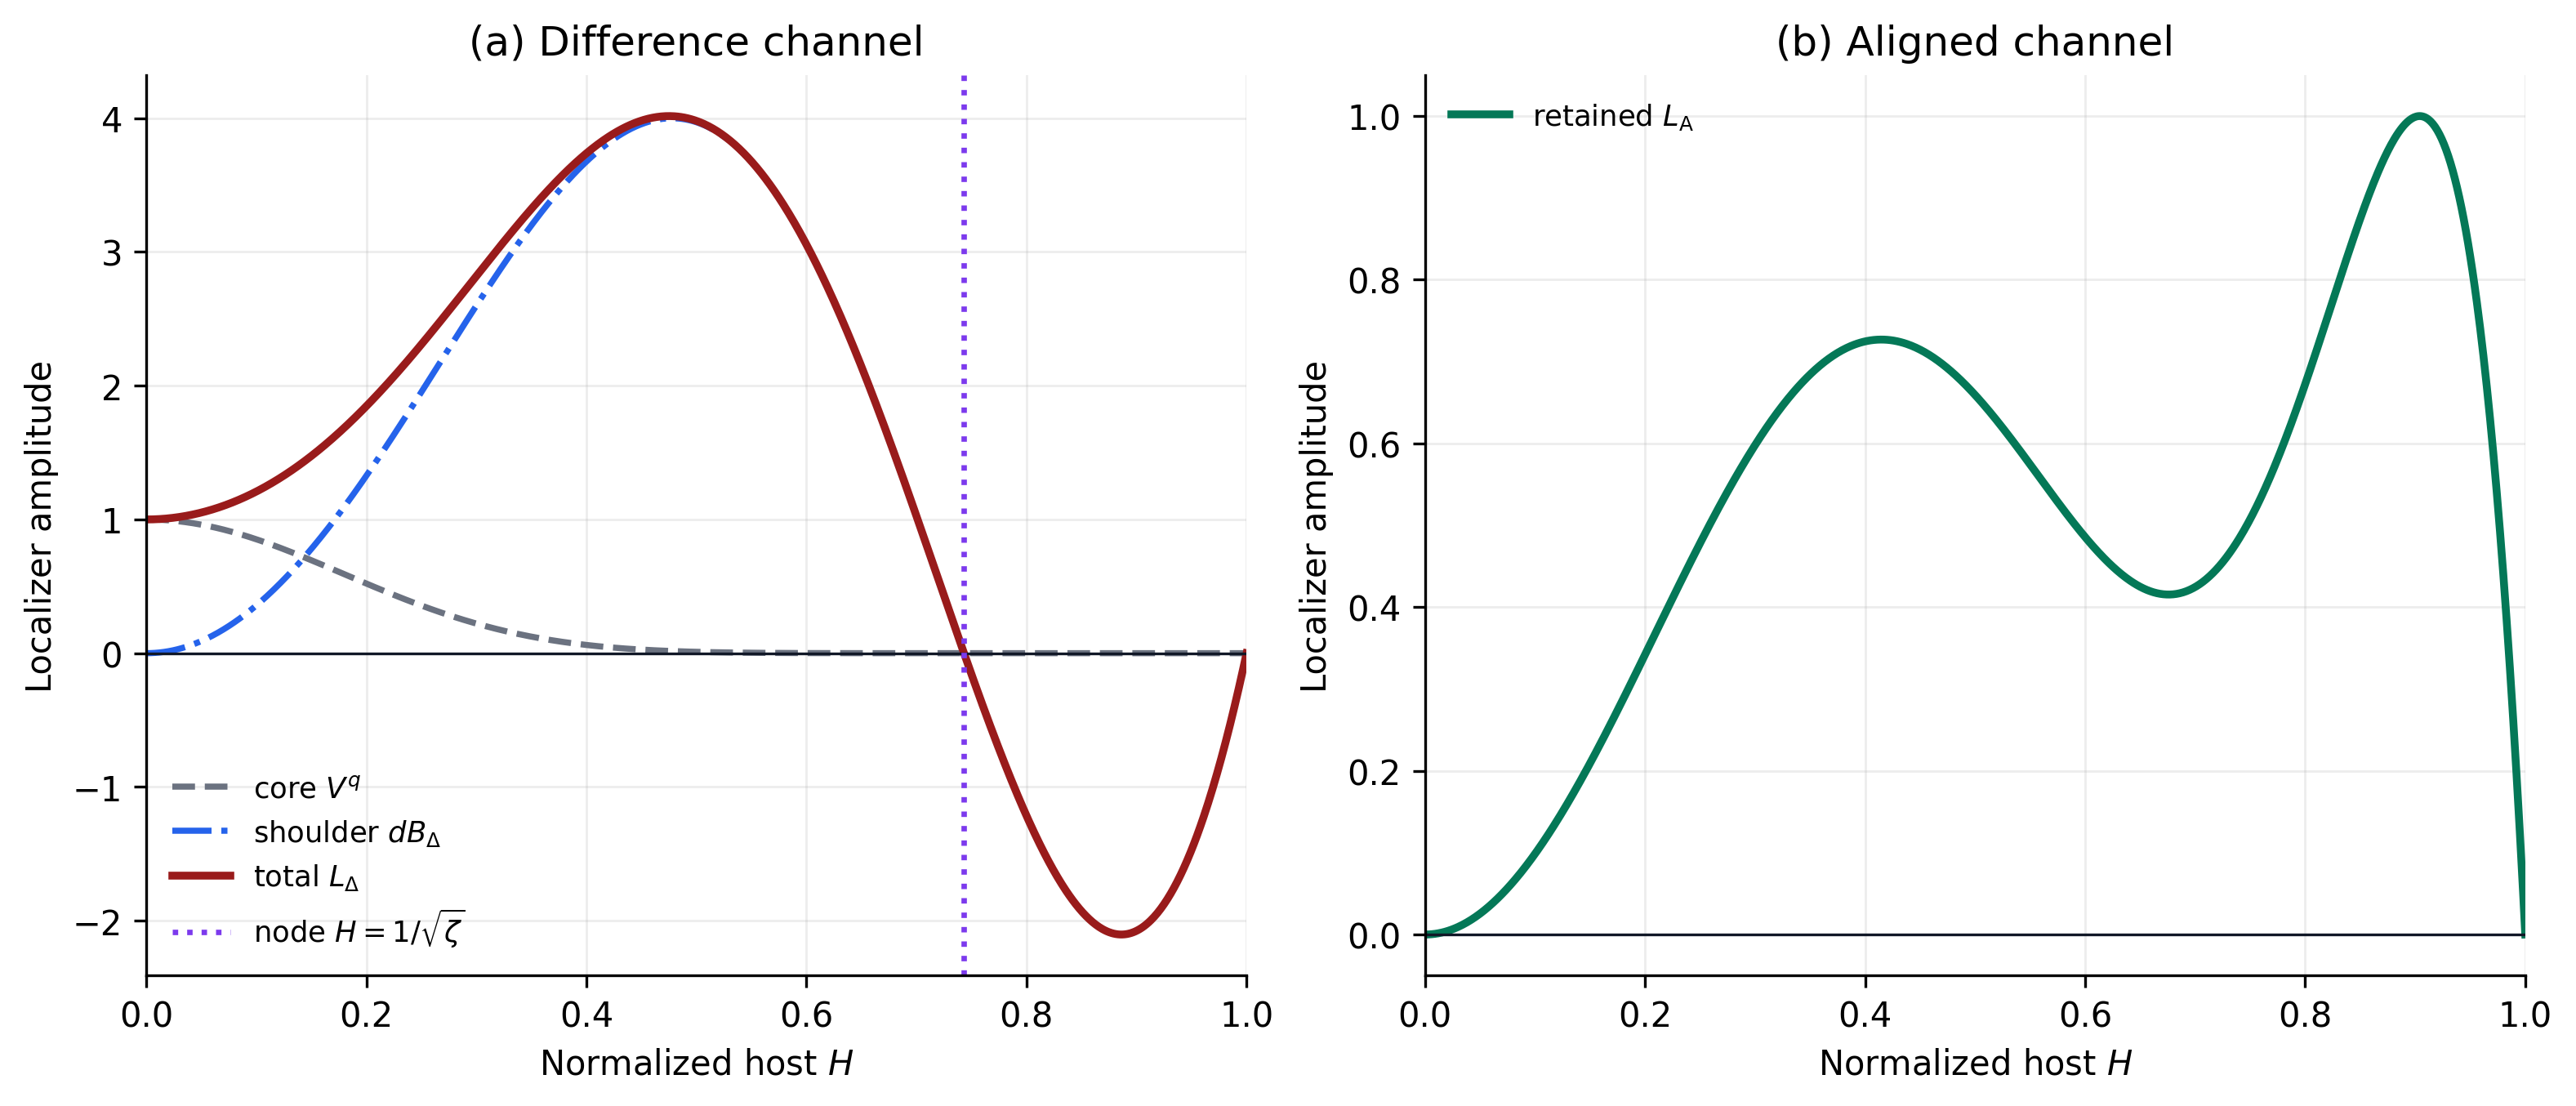
\includegraphics[width=\textwidth]{fixed_background_v0_4_retained_localizers.png}
\caption{Retained checkpoint v0.4 localizers. (a) Difference channel: the central contribution $\vac^q$, sign-changing shoulder $dB_{\Delta}$, and their sum $\ldiff$; the dotted vertical line marks the internal node $\host=1/\sqrt{\zeta}$. (b) Normalized aligned localizer $\lalign$. The curves are functions of the selected parametric ansatz, not independent fundamental fields.}
\label{fig:retained_localizers}
\end{figure}

The directly measured maximum is
\begin{equation}
\boxed{\xibr=2.0934591793773114\times10^{-3}}.
\label{eq:retained_fold}
\end{equation}

The previous checkpoint v0.3 had
\begin{equation}
\xibr^{(0.3)}=2.0682495692869894\times10^{-3}.
\end{equation}
The relative improvement is
\begin{equation}
\frac{\xibr}{\xibr^{(0.3)}}-1
=1.218886\%.
\end{equation}

The new record was obtained after introducing the difference factor $\exp(\lambda\vac^3)$ and directly validating the point $\lambda=-0.35$.

\section{Evolution of the Numerical Record}

The table lists selected retained stages and is not a complete log of all internal slices.

\begin{center}
\small
\begin{tabular}{@{}p{0.34\textwidth}p{0.20\textwidth}p{0.38\textwidth}@{}}
\textbf{Stage} & \textbf{$\xibr$} & \textbf{Role within the ansatz} \\
\hline
One-component core basis & $\approx7.624\times10^{-4}$ & Baseline limit of the preceding one-component sector \\
Connected two-component boundary & $1.278178674\times10^{-3}$ & Introduction of a compensating shoulder \\
Node and difference-width closure & $1.307068707\times10^{-3}$ & Separation of core and shoulder regions \\
Aligned linear width & $1.996071538\times10^{-3}$ & Fine adjustment of the common profile \\
Crossing the $2\times10^{-3}$ benchmark & $2.002226282\times10^{-3}$ & First retained fold above the internal benchmark \\
Polynomial aligned closure v0.3 & $2.068249569287\times10^{-3}$ & Final polynomial profile \\
Difference cubic-exponential v0.4 & $2.093459179377\times10^{-3}$ & Directly confirmed nonpolynomial improvement \\
\end{tabular}
\end{center}

\section{Direct Validation of the Record}

The retained fold has the following diagnostic values:
\begin{align}
\text{predictor relative error} &= 0.057938\%, \\
\text{maximum matching-radius spread} &= 0.074515\%.
\end{align}

Turning points were detected at all three radii. Predictor validation, the matching-radius gate, and the sign-changing fold gate all pass. These tests confirm internal reproducibility of the fold within the selected fixed-background problem, but they do not replace a solution of the fully self-consistent static system with backreaction.

\section{Closure of Nine Coordinates}

A coordinate is called closed when, after local screening and all mandatory physical gates, it does not produce a gain sufficient to authorize a new direct fold calculation. The maximum residual gain of each coordinate is measured relative to the confirmed record.

\begin{center}
\small
\begin{tabular}{@{}p{0.48\textwidth}p{0.18\textwidth}p{0.18\textwidth}@{}}
\textbf{Coordinate} & \textbf{Value} & \textbf{Residual gain} \\
\hline
Difference cubic-exponential tilt $\lambda$ & $-0.35$ & $0.061392\%$ \\
Difference core power $q$ & $16$ & $0.022068\%$ \\
Difference shoulder coefficient $d$ & $4$ & $0.064457\%$ \\
Difference linear width $c_{1,\Delta}$ & $1.20$ & $0.032797\%$ \\
Difference quadratic width $c_{2,\Delta}$ & $0$ & $0.002023\%$ \\
Aligned shell power $p$ & $1$ & $0$ \\
Aligned linear width $c_{1,\mathrm{A}}$ & $-3.260$ & $0.000274\%$ \\
Aligned quadratic width $c_{2,\mathrm{A}}$ & $3.041$ & $0.012141\%$ \\
Aligned cubic-exponential tilt $\rho$ & $0$ & $0.917518\%$ \\
\end{tabular}
\end{center}

All values remain below the threshold in Eq.~\eqref{eq:one_percent_gate}. Therefore, no new direct fold calculation is authorized in the current profile space.

\section{Near-Threshold Aligned Sector}

The aligned factor closest to the threshold is
\begin{equation}
\exp\!\left(\rho\left(1-\host^2\right)^3\right).
\end{equation}

The connected physical branch passes at $\rho=0.29$ and fails the physical gates at $\rho=0.30$. A quadratic fit to the points $\rho=0.26,0.27,0.28$ gives
\begin{align}
\rho_{\mathrm{vertex}} &= 0.269251036968, \\
\xi_{\mathrm{pred}} &= 2.112667042958\times10^{-3}, \\
g_{\mathrm{raw}} &= 0.917518\%, \\
g_{\mathrm{calibrated}} &= 0.859580\%.
\end{align}

The raw gain does not reach $1\%$, so a direct fold calculation was not performed. A separate passing point at $\rho=1$ is excluded because it is separated from the control point by a region in which the physical gates fail. This exclusion prevents disconnected branches from being mixed.

\section{Public Reproducibility}

The compact checkpoint audit is located in
\begin{center}
\texttt{numerics/fixed\_background\_checkpoint\_v0\_4/}.
\end{center}

From the root of the public repository, run
\begin{center}
\texttt{python numerics/fixed\_background\_checkpoint\_v0\_4/audit\_checkpoint.py}.
\end{center}

The expected final output is
\begin{center}
\small
\texttt{PASS: 9/9 audited coordinates closed; retained direct fold=2.093459179377e-03;}

\texttt{maximum unresolved predictor gain=0.917518\%; threshold=1.000000\%}
\end{center}

The audit uses only the Python standard library and checks consistency among derived CSV records. It does not rerun the complete internal boundary-value-solver campaign and is therefore a compact consistency audit rather than an end-to-end release of the primary solver.

\section{Scope Boundaries}

Checkpoint v0.4 establishes only the following:
\begin{enumerate}
\item a directly measured fold exists within the selected fixed-background ansatz, Eq.~\eqref{eq:retained_fold};
\item it is reproduced at three matching radii with a small spread;
\item nine tested coordinates do not authorize another fold under the predeclared rules;
\item the retained configuration can serve as a numerical benchmark for the next independent sector.
\end{enumerate}

Checkpoint v0.4 does not establish:
\begin{enumerate}
\item global optimality over arbitrary functions;
\item a fundamental Field 01 action;
\item full static backreaction;
\item dynamical or nonlinear stability;
\item a physical spectrum of masses, charges, or spins;
\item experimental evidence for a particle, force, or field;
\item the truth of the Field 01 interpretive layer.
\end{enumerate}

\section{Next Authorized Step}

Adding another nearby shape coordinate to the same ansatz is not methodologically justified: all selected directions are closed, and the largest residual gain remains below the direct-validation threshold. The next numerical stage should introduce an independent physical sector with predeclared acceptance gates.

Full static backreaction and dynamic-root analysis are separate programs. They do not follow automatically from the present closure and should begin only after explicit definitions of the variables, equations, admissibility criteria, and computational budget.

\section{Conclusion}

\enlargethispage{2\baselineskip}

Within the restricted fixed-background space of two-component profiles, the checkpoint $\xibr=2.0934591793773114\times10^{-3}$ has been obtained and directly confirmed. The nonpolynomial difference direction improved checkpoint v0.3 by $1.218886\%$, after which all previously optimized coordinates were retested around the new record. Nine coordinates are closed under a common threshold, while the nearest aligned candidate remains $0.082482\%$ below the required predicted gain. The result should be read not as evidence for an ``absolute particle maximum,'' but as a restricted and reproducible benchmark for transition to an independent physical sector.

\begin{thebibliography}{99}

\bibitem{keller1977}
H.~B. Keller,
``Numerical solution of bifurcation and nonlinear eigenvalue problems,''
in \textit{Applications of Bifurcation Theory}, P.~H. Rabinowitz, ed.,
Academic Press, New York, 1977, pp.~359--384.

\bibitem{ascher1995}
U.~M. Ascher, R.~M.~M. Mattheij, and R.~D. Russell,
\textit{Numerical Solution of Boundary Value Problems for Ordinary Differential Equations},
SIAM, Philadelphia, 1995.
\href{https://doi.org/10.1137/1.9781611971231}{doi:10.1137/1.9781611971231}

\bibitem{derrick1964}
G.~H. Derrick,
``Comments on nonlinear wave equations as models for elementary particles,''
\textit{Journal of Mathematical Physics} \textbf{5}, 1252--1254 (1964).
\href{https://doi.org/10.1063/1.1704233}{doi:10.1063/1.1704233}

\bibitem{nielsen1973}
H.~B. Nielsen and P. Olesen,
``Vortex-line models for dual strings,''
\textit{Nuclear Physics B} \textbf{61}, 45--61 (1973).
\href{https://doi.org/10.1016/0550-3213(73)90350-7}{doi:10.1016/0550-3213(73)90350-7}

\bibitem{coleman1985}
S. Coleman,
``Q-balls,''
\textit{Nuclear Physics B} \textbf{262}, 263--283 (1985).
\href{https://doi.org/10.1016/0550-3213(85)90286-X}{doi:10.1016/0550-3213(85)90286-X}

\bibitem{vakhitov1973}
N.~G. Vakhitov and A.~A. Kolokolov,
``Stationary solutions of the wave equation in a medium with nonlinearity saturation,''
\textit{Radiophysics and Quantum Electronics} \textbf{16}, 783--789 (1973).
\href{https://doi.org/10.1007/BF01031343}{doi:10.1007/BF01031343}

\end{thebibliography}

\end{document}